\documentclass[11pt,letterpaper]{article}

% ============================================================================
% PACKAGES
% ============================================================================
\usepackage[utf8]{inputenc}
\usepackage[T1]{fontenc}
\usepackage{helvet}
\renewcommand{\familydefault}{\sfdefault}
\usepackage[margin=0.85in, headheight=28pt]{geometry}
\usepackage{graphicx}
\usepackage{xcolor}
\usepackage{tikz}
\usepackage{tcolorbox}
\usepackage{booktabs}
\usepackage{enumitem}
\usepackage{hyperref}
\usepackage{fancyhdr}
\usepackage{titlesec}
\usepackage{multicol}
\usepackage{listings}
\usepackage{upquote}
\usepackage{amsmath,amssymb}
\usepackage{pgfplots}
\usepackage{array}
\usepackage{longtable}

% Ragged-right paragraph columns to prevent word spacing issues
\newcolumntype{L}[1]{>{\raggedright\arraybackslash}p{#1}}

% Increase vertical spacing between table rows for readability
\renewcommand{\arraystretch}{1.4}
\usepackage{colortbl}
\usepackage{pifont}
\usepackage{setspace}
\usepackage{parskip}
\usepackage{caption}
\usepackage{tabularx}

\pgfplotsset{compat=1.18}
\usetikzlibrary{shapes.geometric, arrows.meta, positioning, calc, decorations.pathreplacing, backgrounds, fit, shadows.blur, matrix, patterns, fadings, shadings}

% ============================================================================
% COLOR DEFINITIONS - Institutional Research Theme
% ============================================================================
\definecolor{instdark}{HTML}{1C2833}
\definecolor{instnavy}{HTML}{2C3E50}
\definecolor{instblue}{HTML}{34495E}
\definecolor{instaccent}{HTML}{5D6D7E}
\definecolor{instgold}{HTML}{B7950B}
\definecolor{instslate}{HTML}{566573}
\definecolor{successgreen}{HTML}{1E8449}
\definecolor{warningamber}{HTML}{B9770E}
\definecolor{alertcoral}{HTML}{922B21}
\definecolor{infocyan}{HTML}{1A5276}
\definecolor{coolgray}{HTML}{7B7D7D}
\definecolor{lightgray}{HTML}{EAECEE}
\definecolor{codebg}{HTML}{F4F6F7}
\definecolor{codetext}{HTML}{2C3E50}
\definecolor{gridlight}{HTML}{D5D8DC}
\definecolor{nodecyan}{HTML}{2E86AB}
\definecolor{nodeorange}{HTML}{D35400}
\definecolor{nodegreen}{HTML}{27AE60}
\definecolor{nodepurple}{HTML}{8E44AD}

% ============================================================================
% HYPERREF SETUP
% ============================================================================
\hypersetup{
  colorlinks=true,
  linkcolor=instnavy,
  urlcolor=instaccent,
  pdftitle={AI Agents and Institutional Erosion of Intelligence Monopolies},
  pdfauthor={Emerging Technology Risk Assessment}
}

% ============================================================================
% SPACING AND TYPOGRAPHY
% ============================================================================
\setstretch{1.15}
\setlength{\parskip}{0.5em}
\setlist{nosep, leftmargin=1.5em, itemsep=0.3em}

% ============================================================================
% PAGE STYLE - Minimal with data grid accent
% ============================================================================
\pagestyle{fancy}
\fancyhf{}
\fancyhead[L]{%
  \begin{tikzpicture}[baseline=-0.5ex]
    % Mini data grid
    \foreach \x in {0,0.12,0.24,0.36,0.48} {
      \foreach \y in {0,0.12,0.24} {
        \fill[instaccent, opacity=0.3] (\x,\y) circle (0.03);
      }
    }
  \end{tikzpicture}
  \hspace{0.5em}\textcolor{instnavy}{\textsf{\small ETRA-2026-IC-001}}%
}
\fancyhead[R]{\textcolor{coolgray}{\textsf{\thepage}}}
\fancyfoot[C]{\textcolor{coolgray}{\footnotesize\textsf{Emerging Technology Risk Assessment \textbar{} Projection Report}}}
\renewcommand{\headrulewidth}{0pt}
\renewcommand{\footrulewidth}{0pt}

\fancyheadoffset{0pt}
\setlength{\headheight}{32pt}

% ============================================================================
% SECTION FORMATTING - Clean institutional style
% ============================================================================
\titleformat{\section}
  {\normalfont\LARGE\bfseries\color{instdark}}
  {\thesection}{0.8em}{}[\vspace{-0.3em}{\color{gridlight}\rule{\textwidth}{1pt}}]
\titleformat{\subsection}
  {\normalfont\Large\bfseries\color{instnavy}}
  {\thesubsection}{0.6em}{}
\titleformat{\subsubsection}
  {\normalfont\large\color{instslate}\bfseries}
  {\thesubsubsection}{0.5em}{}

\titlespacing*{\section}{0pt}{3ex plus 1ex minus .2ex}{2ex plus .2ex}
\titlespacing*{\subsection}{0pt}{2.5ex plus 1ex minus .2ex}{1.5ex plus .2ex}

\setcounter{tocdepth}{2}

% ============================================================================
% TCOLORBOX ENVIRONMENTS
% ============================================================================
\tcbuselibrary{skins,breakable,hooks}

\newtcolorbox{keybox}[1][Key Finding]{
  enhanced, breakable,
  colback=instblue!5, colframe=instblue,
  colbacktitle=instblue, coltitle=white,
  fonttitle=\bfseries\sffamily,
  title={\ding{72}\hspace{0.5em}#1},
  boxrule=0pt, leftrule=3pt, arc=0pt, outer arc=0pt,
  left=12pt, right=12pt, top=8pt, bottom=8pt
}

\newtcolorbox{warnbox}[1][Warning]{
  enhanced, breakable,
  colback=warningamber!8, colframe=warningamber,
  colbacktitle=warningamber, coltitle=white,
  fonttitle=\bfseries\sffamily,
  title={\ding{74}\hspace{0.5em}#1},
  boxrule=0pt, leftrule=3pt, arc=0pt, outer arc=0pt,
  left=12pt, right=12pt, top=8pt, bottom=8pt
}

\newtcolorbox{criticalbox}[1][Critical]{
  enhanced, breakable,
  colback=alertcoral!8, colframe=alertcoral,
  colbacktitle=alertcoral, coltitle=white,
  fonttitle=\bfseries\sffamily,
  title={\ding{74}\hspace{0.5em}#1},
  boxrule=0pt, leftrule=3pt, arc=0pt, outer arc=0pt,
  left=12pt, right=12pt, top=8pt, bottom=8pt
}

\newtcolorbox{recbox}[1][Recommendation]{
  enhanced, breakable,
  colback=successgreen!8, colframe=successgreen,
  colbacktitle=successgreen, coltitle=white,
  fonttitle=\bfseries\sffamily,
  title={\ding{51}\hspace{0.5em}#1},
  boxrule=0pt, leftrule=3pt, arc=0pt, outer arc=0pt,
  left=12pt, right=12pt, top=8pt, bottom=8pt
}

\newtcolorbox{infobox}[1][Note]{
  enhanced, breakable,
  colback=infocyan!8, colframe=infocyan,
  colbacktitle=infocyan, coltitle=white,
  fonttitle=\bfseries\sffamily,
  title={\ding{73}\hspace{0.5em}#1},
  boxrule=0pt, leftrule=3pt, arc=0pt, outer arc=0pt,
  left=12pt, right=12pt, top=8pt, bottom=8pt
}

\newtcolorbox{defbox}[1][Definition]{
  enhanced, breakable,
  colback=instgold!8, colframe=instgold,
  colbacktitle=instgold!90!black, coltitle=white,
  fonttitle=\bfseries\sffamily,
  title={\ding{70}\hspace{0.5em}#1},
  boxrule=0pt, leftrule=3pt, arc=0pt, outer arc=0pt,
  left=12pt, right=12pt, top=8pt, bottom=8pt
}

\newtcolorbox{scenariobox}[1][Scenario]{
  enhanced, breakable,
  colback=instslate!5, colframe=instslate,
  colbacktitle=instslate, coltitle=white,
  fonttitle=\bfseries\sffamily,
  title={\ding{118}\hspace{0.5em}#1},
  boxrule=0pt, leftrule=3pt, arc=0pt, outer arc=0pt,
  left=12pt, right=12pt, top=8pt, bottom=8pt
}

% ============================================================================
% DOCUMENT
% ============================================================================
\begin{document}

% ============================================================================
% TITLE PAGE - Network Topology Visualization
% ============================================================================
\begin{titlepage}

\begin{tikzpicture}[remember picture, overlay]
  % Background gradient
  \fill[instdark] (current page.north west) rectangle (current page.south east);

  % Abstract data grid background (right side)
  \begin{scope}[shift={(current page.center)}, opacity=0.08]
    \foreach \x in {2,2.8,...,10} {
      \foreach \y in {-12,-11.2,...,12} {
        \fill[white] (\x,\y) circle (0.06);
      }
    }
  \end{scope}

  % Main network visualization - verification/collection pivot concept
  \begin{scope}[shift={([xshift=-0.5cm, yshift=3.5cm]current page.center)}]
    % Outer ring nodes - IC agencies and functions
    \foreach \angle/\col/\label in {
      30/nodecyan/ODNI,
      75/nodegreen/CIA,
      120/nodeorange/NSA,
      165/nodepurple/FBI,
      210/nodecyan/DIA,
      255/nodegreen/NGA,
      300/nodeorange/DHS,
      345/nodepurple/DOE
    } {
      % Node
      \fill[\col, opacity=0.9] (\angle:4.5cm) circle (0.4cm);
      \node[white, font=\fontsize{5}{5}\selectfont\bfseries] at (\angle:4.5cm) {\label};
      % Connection to center
      \draw[\col, opacity=0.4, line width=1pt] (0,0) -- (\angle:4cm);
      % Outer data points
      \foreach \r in {5.2,5.6,6} {
        \fill[\col, opacity=0.2] (\angle:\r cm) circle (0.08);
      }
    }

    % Inner ring - verification layers
    \foreach \angle/\col in {0/nodecyan, 45/nodegreen, 90/nodeorange, 135/nodepurple, 180/nodecyan, 225/nodegreen, 270/nodeorange, 315/nodepurple} {
      \fill[\col, opacity=0.6] (\angle:2.5cm) circle (0.2cm);
      \draw[\col, opacity=0.3, line width=0.5pt] (\angle:2.5cm) -- ({(\angle+45)}:2.5cm);
    }

    % Central hub - The Verification Pivot
    \fill[white, opacity=0.1] (0,0) circle (1.8cm);
    \fill[white, opacity=0.15] (0,0) circle (1.4cm);
    \fill[instgold] (0,0) circle (0.8cm);
    \node[instdark, font=\fontsize{7}{7}\selectfont\bfseries] at (0,0.15) {VERIFY};
    \node[instdark, font=\fontsize{7}{7}\selectfont\bfseries] at (0,-0.15) {PIVOT};

    % Cross-connections (showing complexity)
    \draw[white, opacity=0.1, line width=0.5pt] (30:4cm) -- (165:4cm);
    \draw[white, opacity=0.1, line width=0.5pt] (75:4cm) -- (255:4cm);
    \draw[white, opacity=0.1, line width=0.5pt] (120:4cm) -- (300:4cm);
    \draw[white, opacity=0.1, line width=0.5pt] (210:4cm) -- (345:4cm);
  \end{scope}

  % Document classification bar
  \fill[instgold] ([yshift=-1.5cm]current page.north west) rectangle ([yshift=-2.2cm]current page.north east);
  \node[instdark, font=\small\bfseries\sffamily] at ([yshift=-1.85cm]current page.north) {PROJECTION REPORT \textbar{} ETRA-2026-IC-001 \textbar{} JANUARY 2026};

  % Title block (bottom left)
  \node[anchor=south west, text width=14cm] at ([xshift=1.5cm, yshift=3cm]current page.south west) {
    {\fontsize{11}{13}\selectfont\color{instgold}\sffamily EMERGING TECHNOLOGY RISK ASSESSMENT}\\[0.8cm]
    {\fontsize{32}{38}\selectfont\bfseries\color{white}AI Agents and}\\[0.2cm]
    {\fontsize{32}{38}\selectfont\bfseries\color{white}Institutional Erosion of}\\[0.2cm]
    {\fontsize{32}{38}\selectfont\bfseries\color{white}Intelligence Monopolies}\\[0.6cm]
    {\large\color{gridlight}\sffamily The Verification Pivot: How Autonomous AI Transforms the IC}
  };

  % Metadata block (bottom right)
  \node[anchor=south east, text width=5cm, align=right] at ([xshift=-1.5cm, yshift=3cm]current page.south east) {
    \color{instaccent}\small\sffamily
    \textbf{Document Type:} Projection\\[0.2em]
    \textbf{Time Horizon:} 2026--2030\\[0.2em]
    \textbf{Classification:} Policy Research\\[0.2em]
    \textbf{Version:} 0.1 (Initial Draft)
  };

  % Vertical accent line
  \draw[instgold, line width=2pt] ([xshift=1.5cm, yshift=3cm]current page.south west) -- ([xshift=1.5cm, yshift=10.5cm]current page.south west);

\end{tikzpicture}
\end{titlepage}

% ============================================================================
% EXECUTIVE SUMMARY
% ============================================================================
\thispagestyle{empty}
\vspace*{0.5cm}

% Mini header visualization
\noindent\begin{tikzpicture}
  \fill[instdark] (0,0) rectangle (\textwidth, 0.15);
  \foreach \x in {0.5,1,...,16.5} {
    \fill[instgold, opacity=0.5] (\x, 0.075) circle (0.04);
  }
\end{tikzpicture}

\vspace{0.5cm}
\begin{center}
{\color{instdark}\Large\bfseries Executive Summary}
\end{center}
\vspace{0.3cm}

\begin{tcolorbox}[enhanced, colback=lightgray, colframe=instblue!50, boxrule=1pt, arc=3pt,
  left=10pt, right=10pt, top=10pt, bottom=10pt]
This projection examines how autonomous AI agents are eroding the traditional advantages of national intelligence communities, particularly the U.S. Intelligence Community (IC). We analyze current technological capabilities as of early 2026, project likely institutional impacts through 2030, and examine how intelligence organizations must adapt to maintain epistemic authority in an AI-saturated information environment.
\end{tcolorbox}

\vspace{0.5cm}

\begin{keybox}[Central Thesis: The Verification Pivot]
The IC is transitioning from an era of \textbf{Information Scarcity}---where advantage derived from superior collection capabilities---to an era of \textbf{Epistemic Contamination}---where advantage derives from superior verification capabilities. This represents the most significant shift in intelligence dynamics since the advent of signals intelligence.

\vspace{0.5em}
\textbf{Secondary Thesis: From Secrecy to Provenance}

In an AI-saturated environment, \textit{classification alone} is no longer a reliable proxy for decision value. Intelligence products derive value from (1) protecting sources and methods \textit{and} (2) providing high-integrity, auditable provenance for key claims.
\end{keybox}

\vspace{0.5cm}

\begin{keybox}[Key Findings]
\begin{enumerate}
  \item \textbf{[E] The Democratization of Tradecraft}: AI agents have effectively ``automated the Handler.'' Tradecraft that once required sovereign state infrastructure is now a commodity.
  \item \textbf{[E]} The IC faces a dual crisis: \textbf{Process DoS} (investigative capacity overwhelmed) and an \textbf{Attribution-Intent Gap} (inability to establish human intent behind agent actions)
  \item \textbf{[E]} Current collection-centric metrics become counterproductive in an environment of epistemic contamination
  \item \textbf{[S]} Success in 2026-2030 will be measured by the ability to maintain an ``Epistemic Clean Room''---a verified environment for decision-making
  \item \textbf{[E]} The ``Plausible Deniability 2.0'' dynamic will strain existing legal frameworks for state responsibility
  \item \textbf{[S]} Without adaptation, the IC risks becoming a high-cost verification bottleneck rather than a strategic advantage
\end{enumerate}
\end{keybox}

\vspace{0.5cm}

\begin{warnbox}[Scope Limitations]
This document analyzes capabilities and institutional dynamics for defensive policy purposes. It does not provide operational guidance and explicitly omits technical implementation details that could enable harm. Analysis focuses on how autonomous agents change intelligence dynamics, not on intelligence methods generally.
\end{warnbox}

\vspace{0.5cm}

% ============================================================================
% COMMITTEE TAKEAWAYS
% ============================================================================
\begin{center}
{\color{instdark}\Large\bfseries Committee Takeaways}
\end{center}

\begin{defbox}[5 Non-Negotiable Assumptions]
\begin{enumerate}
  \item \textbf{The capability floor has risen permanently} --- Low-cost access to frontier models can automate major components of tradecraft---research, targeting, persona drafting, multilingual engagement---reducing manpower barriers even when operational constraints remain.
  \item \textbf{Collection without verification is now a liability} --- In targeted collection environments, agent-generated decoys could plausibly outnumber authentic human signals by $\sim$3--30$\times$. Traditional signal-to-noise filters become unreliable.
  \item \textbf{Attribution of intent is structurally harder} --- The ``Delegation Defense'' (blaming autonomous agent behavior) provides plausible deniability for state actors using AI agents.
  \item \textbf{Institutional speed cannot match adversary iteration} --- Adversaries iterate at software speed; IC adoption is constrained by procurement, authorities, and assurance requirements.
  \item \textbf{[O] Verification workforce is contracting} --- Public reporting indicates significant IC staffing reductions concurrent with rising verification demands.
\end{enumerate}
\end{defbox}

\vspace{0.3cm}

\begin{keybox}[5 Most Likely Impact Paths]
\begin{center}
\small
\begin{tabular}{L{3cm}L{5cm}L{4.5cm}}
\toprule
\textbf{Path} & \textbf{Mechanism} & \textbf{Primary Victims} \\
\midrule
Process DoS & Agent-generated leads, hyper-specific FOIA requests, synthetic tips overwhelm capacity & FBI, DHS, investigative agencies \\
Epistemic Contamination & Synthetic content pollutes OSINT/GEOINT, eroding ``ground truth'' & All-source analysts, ODNI \\
Attribution-Intent Gap & States claim agents ``autonomously derived'' criminal methods & Legal/policy leadership, State Dept \\
Algorithmic Capture & Compromise of AI systems used by leadership biases intelligence products & ODNI, CIA, NSC \\
Nano-Smurfing Evasion & Sub-threshold procurement of dual-use items evades monitoring & Treasury, DOE, proliferation watchers \\
\bottomrule
\end{tabular}
\end{center}
\end{keybox}

\vspace{0.3cm}

\begin{infobox}[Success Criteria]
\begin{center}
\small
\begin{tabular}{L{4cm}L{4.2cm}L{4.2cm}}
\textbf{90 days} & \textbf{180 days} & \textbf{1 year} \\
\midrule
Verification metric defined; red-teams run; no unvetted AI in leadership workflows & Provenance prototype; detection sharing operational & Verification scales with collection; international coordination initiated \\
\end{tabular}
\end{center}
\end{infobox}

\vspace{0.5cm}

% ============================================================================
% BASE-RATE CONTEXT
% ============================================================================
\begin{center}
{\color{instdark}\Large\bfseries Base-Rate Context: Anchoring Expectations}
\end{center}

\vspace{0.3cm}

\textbf{To prevent fear-driven misreading, we anchor expectations in historical reality.}

The Intelligence Community has repeatedly adapted to technological disruption. The question is not \textit{whether} it can adapt, but whether current adaptation is \textit{fast enough} given the pace of AI capability development.

\begin{center}
\small
\begin{tabular}{L{2.5cm}L{10cm}}
\toprule
\textbf{Era} & \textbf{Adaptation} \\
\midrule
1940s-50s & Transition from HUMINT-dominated to SIGINT-integrated operations \\
1970s-80s & Adaptation to satellite imagery and global communications intercept \\
1990s-2000s & Integration of open-source intelligence and digital collection \\
2010s & Response to social media, encrypted communications, and cyber operations \\
\bottomrule
\end{tabular}
\end{center}

\begin{warnbox}[The AI Transition Differs in Three Critical Ways]
\begin{enumerate}
  \item \textbf{Speed}: Previous transitions unfolded over decades; AI capabilities iterate weekly
  \item \textbf{Accessibility}: Previous capabilities required state resources; AI agents are commercially available
  \item \textbf{Attribution}: Previous threats had identifiable human operators; AI agents create intent ambiguity
\end{enumerate}
\end{warnbox}

\begin{infobox}[What This Document Does NOT Claim]
\begin{itemize}
  \item We do not claim the IC is currently failing---many adaptation efforts are underway
  \item We do not claim AI agents make traditional intelligence obsolete---human judgment remains essential
  \item We do not claim all projected scenarios are equally likely---probability varies significantly
  \item We do not claim adversaries have fully operationalized these capabilities---but the trajectory is clear
\end{itemize}
\end{infobox}

\newpage
\tableofcontents
\newpage

% ============================================================================
% PART I - Foundations
% ============================================================================
\clearpage
\thispagestyle{empty}
\vspace*{-0.85in}
\noindent\hspace*{-0.85in}\begin{tikzpicture}
  % Header background
  \fill[instdark] (0,0) rectangle (\paperwidth, -10cm);

  % Part label and title
  \node[instgold, font=\fontsize{10}{10}\selectfont\sffamily] at (0.5\paperwidth, -1.2cm) {PART I};
  \node[white, font=\fontsize{48}{48}\selectfont\bfseries] at (0.5\paperwidth, -2.8cm) {Foundations};
  \node[white, opacity=0.7, font=\normalsize\sffamily] at (0.5\paperwidth, -4.2cm) {Theory, Context, and Conceptual Framework};

  % Era transition visualization
  \begin{scope}[shift={(4cm, -7.5cm)}]
    % Collection Era (left)
    \fill[alertcoral, opacity=0.7] (0, 0) circle (1.2cm);
    \node[white, font=\fontsize{8}{8}\selectfont\bfseries] at (0, 0.2) {COLLECTION};
    \node[white, font=\fontsize{6}{6}\selectfont] at (0, -0.2) {ERA};
    \node[white, opacity=0.7, font=\fontsize{7}{7}\selectfont] at (0, -1.7) {Information Scarcity};

    % Arrow
    \draw[instgold, line width=4pt, -Stealth] (1.8, 0) -- (4.2, 0);
    \node[instgold, font=\fontsize{9}{9}\selectfont\bfseries] at (3, 0.6) {PIVOT};

    % Verification Era (right)
    \fill[successgreen, opacity=0.8] (6, 0) circle (1.2cm);
    \node[white, font=\fontsize{8}{8}\selectfont\bfseries] at (6, 0.2) {VERIFY};
    \node[white, font=\fontsize{6}{6}\selectfont] at (6, -0.2) {ERA};
    \node[white, opacity=0.7, font=\fontsize{7}{7}\selectfont] at (6, -1.7) {Epistemic Contamination};
  \end{scope}

  % Threat tier visualization (right side)
  \begin{scope}[shift={(13cm, -7cm)}]
    \node[white, opacity=0.5, font=\fontsize{7}{7}\selectfont] at (1.5, 1.5) {CAPABILITY FLOOR RISE};

    % Bars showing tier compression
    \fill[instaccent, opacity=0.4] (0, 0) rectangle (0.6, 0.5);
    \fill[instaccent, opacity=0.5] (0.8, 0) rectangle (1.4, 1.0);
    \fill[instaccent, opacity=0.6] (1.6, 0) rectangle (2.2, 1.5);
    \fill[instgold, opacity=0.8] (2.4, 0) rectangle (3.0, 2.2);

    \node[white, opacity=0.6, font=\fontsize{5}{5}\selectfont] at (0.3, -0.3) {T0};
    \node[white, opacity=0.6, font=\fontsize{5}{5}\selectfont] at (1.1, -0.3) {T1};
    \node[white, opacity=0.6, font=\fontsize{5}{5}\selectfont] at (1.9, -0.3) {T2};
    \node[white, opacity=0.6, font=\fontsize{5}{5}\selectfont] at (2.7, -0.3) {T3+};
  \end{scope}

  % Bottom accent
  \fill[instgold] (2cm, -9.2cm) rectangle (\paperwidth-2cm, -9.3cm);
\end{tikzpicture}

\vspace{0.8cm}
\begin{center}
\begin{minipage}{0.9\textwidth}
\begin{tcolorbox}[enhanced, colback=white, colframe=instblue!30, boxrule=1pt, arc=4pt,
  left=15pt, right=15pt, top=12pt, bottom=12pt]
\textcolor{instdark}{\textbf{Sections Covered}}
\vspace{0.4em}
\begin{itemize}[nosep]
  \item \textbf{Section 1}: Introduction and Methodology
  \item \textbf{Section 2}: Definitions and Conceptual Framework
  \item \textbf{Section 3}: Theoretical Framework: The Monopoly Erosion Model
\end{itemize}
\end{tcolorbox}
\end{minipage}
\end{center}

\vspace{0.8cm}

\section{Introduction and Methodology}

\subsection{Purpose}

The U.S. Intelligence Community has maintained strategic advantage through superior capabilities in collection, analysis, and dissemination of information. This advantage rested on a fundamental asymmetry: the IC could gather and process information at scales and speeds that adversaries and non-state actors could not match.

AI agents erode this asymmetry. This projection analyzes how that erosion manifests across the 18-agency IC, what institutional adaptations are required, and what metrics should guide the transition from collection-centric to verification-centric intelligence operations.

\subsection{Relationship to Other ETRA Reports}

This report builds on and complements other documents in the Emerging Technology Risk Assessment series:

\begin{center}
\small
\begin{tabular}{L{4.5cm}L{3cm}L{6cm}}
\toprule
\textbf{Report} & \textbf{Document ID} & \textbf{Relationship} \\
\midrule
AI Agents as Economic Actors & ETRA-2025-AEA-001 & Establishes baseline agent capabilities \\
AI Agents and Financial Integrity & ETRA-2025-FIN-001 & Details nano-smurfing and evasion \\
AI Agents and Espionage Operations & ETRA-2025-ESP-001 & Covers adversary HUMINT augmentation \\
AI Agents and Political Targeting & ETRA-2025-POL-001 & Addresses targeting of leadership \\
\bottomrule
\end{tabular}
\end{center}

\subsection{Methodology}

This analysis draws on:
\begin{itemize}
  \item \textbf{Current capability assessment} of AI agent systems as deployed in late 2025/early 2026
  \item \textbf{Institutional analysis} of IC structure, incentives, and historical adaptation patterns
  \item \textbf{Open-source intelligence} on adversary AI adoption and doctrine
  \item \textbf{Expert consultation} across intelligence studies, AI safety, and national security law
  \item \textbf{Red team exercises} examining IC vulnerability to agent-enabled operations
\end{itemize}

We deliberately avoid classified information, specific operational details that could enable harm, named targeting scenarios, and technical implementation details for adversarial applications.

\subsection{Epistemic Status Markers}

\begin{defbox}[Epistemic Status Markers]
Throughout this document, claims are tagged with confidence levels:

\vspace{0.5em}
\begin{tabular}{L{1.2cm}L{3.5cm}L{8cm}}
\textbf{[O]} & Open-source documented & Direct public documentation supports this specific claim \\
\textbf{[D]} & Data point & Specific quantified measurement with citation \\
\textbf{[E]} & Expert judgment & Supported by expert consensus, analogies, or partial evidence \\
\textbf{[S]} & Speculative projection & Forward projection with significant uncertainty \\
\end{tabular}
\end{defbox}

\section{Definitions and Conceptual Framework}

\subsection{Core Definitions}

\begin{defbox}[Core Definitions]
\textbf{AI Agent}: An AI system capable of autonomous multi-step task execution, tool use, and goal-directed behavior with minimal human oversight per action.

\vspace{0.5em}
\textbf{Intelligence Community (IC)}: The 18 U.S. government agencies responsible for intelligence activities, coordinated by ODNI.

\vspace{0.5em}
\textbf{Epistemic Contamination}: A state where the information environment contains sufficient synthetic or manipulated content that establishing ``ground truth'' requires significant verification resources.

\vspace{0.5em}
\textbf{Process DoS}: Overwhelming an organization's investigative capacity with plausible-but-false leads, requests, or data.

\vspace{0.5em}
\textbf{Attribution-Intent Gap}: The structural difficulty of establishing human intent when actions are executed by autonomous agents.

\vspace{0.5em}
\textbf{Verification Latency}: The time required to establish whether intelligence is authentic, synthetic, or manipulated.
\end{defbox}

\subsection{The Threat Actor Taxonomy (T0-T4)}

\begin{center}
\small
\begin{tabular}{L{1cm}L{3cm}L{4cm}L{5cm}}
\toprule
\textbf{Tier} & \textbf{Actor Class} & \textbf{Pre-Agent Capability} & \textbf{Post-Agent Capability} \\
\midrule
T0 & Individual hobbyist & Basic OSINT & Automated OSINT synthesis \\
T1 & Skilled individual & Targeted research, manual SE & Persistent personas, multi-channel \\
T2 & Organized crime & Coordinated operations & Agent swarms, financial structuring \\
T3 & Regional state & Dedicated intel programs & Scaled automation \\
T4 & Major state actor & Full-spectrum capabilities & AI-augmented full-spectrum \\
\bottomrule
\end{tabular}
\end{center}

\begin{keybox}[Key Insight]
The gap between T0-T2 and T3-T4 has compressed. A T1 actor with agent capabilities can now execute tradecraft that previously required T3 resources.
\end{keybox}

\subsection{The Intelligence Disciplines (INTs)}

\begin{center}
\small
\begin{tabular}{L{1.5cm}L{3cm}L{3cm}L{5cm}}
\toprule
\textbf{INT} & \textbf{Full Name} & \textbf{Primary Method} & \textbf{AI Vulnerability Vector} \\
\midrule
HUMINT & Human Intelligence & Human sources & Synthetic personas, handler overload \\
SIGINT & Signals Intelligence & Communications intercept & Traffic shaping, encryption automation \\
OSINT & Open-Source Intelligence & Public information & Content pollution, synthetic media \\
GEOINT & Geospatial Intelligence & Imagery and mapping & Synthetic imagery, decoy generation \\
MASINT & Measurement \& Signature & Technical sensors & Sensor spoofing, signature mimicry \\
FININT & Financial Intelligence & Money flows & Nano-smurfing, shell automation \\
\bottomrule
\end{tabular}
\end{center}

\section{Theoretical Framework: The Monopoly Erosion Model}

\subsection{Capability Floor Elevation [E]}

\textbf{The Core Dynamic}: Non-state actors can now leverage AI agents to execute tradecraft that previously required sovereign state resources. This represents a structural change in the distribution of intelligence capabilities.

\begin{center}
\small
\begin{tabular}{L{2cm}L{4cm}L{6cm}}
\toprule
\textbf{Era} & \textbf{Monopoly Basis} & \textbf{Barrier to Entry} \\
\midrule
Pre-WWII & Human networks, diplomatic access & Time, trust, language \\
Cold War & SIGINT infrastructure, satellites & Capital (\$billions), technical expertise \\
Post-9/11 & Fusion centers, data access & Legal authority, data pipelines \\
2020s & AI processing, verification & \textbf{Collapsing} \\
\bottomrule
\end{tabular}
\end{center}

\begin{infobox}[Floor Up, Ceiling Up]
The full picture is more complex:
\begin{itemize}
  \item \textbf{Floor rises}: Non-state actors gain access to previously state-level tradecraft
  \item \textbf{Ceiling rises too}: State actors also gain agents + proprietary data + dedicated hardware
  \item \textbf{Verification is also an AI race}: Defensive tooling benefits from AI acceleration
\end{itemize}
The compression is real but not uniform. State actors retain advantages in classified datasets, compute infrastructure, and legal authorities.
\end{infobox}

\subsection{Physical World Friction [E]}

\begin{center}
\small
\begin{tabular}{L{3.5cm}L{2.5cm}L{7cm}}
\toprule
\textbf{Domain} & \textbf{Friction Level} & \textbf{What Agents Enable} \\
\midrule
Cognitive automation & Low & Research, drafting, translation, pattern recognition \\
Digital operations & Medium & Network reconnaissance, social engineering \\
Physical/logistics & High & Procurement, movement, material acquisition \\
\bottomrule
\end{tabular}
\end{center}

Agents dramatically accelerate cognitive and many digital operations. Physical operations retain significant friction---OPSEC, logistics, border crossings. This distinction matters: most scenarios involve cognitive and digital threats.

\subsection{The Collection-to-Verification Pivot [E]}

\textbf{The Historical Advantage}: The IC's traditional advantage was ``The Intercept''---the ability to collect signals that adversaries could not protect.

\textbf{The 2026 Reality}: In targeted collection environments, agent-generated decoys could plausibly outnumber authentic human signals by 3--30x. Traditional signal-to-noise filters become unreliable.

\textbf{The New Advantage}: In an era of epistemic contamination, advantage comes from ``The Provenance''---the ability to establish authenticity, trace origins, and verify claims.

\begin{keybox}[Metrics Inversion]
\begin{center}
\small
\begin{tabular}{L{5.5cm}L{6cm}}
\textbf{Old Metric (Collection Era)} & \textbf{New Metric (Verification Era)} \\
\midrule
Signals collected per day & Signals verified per day \\
Sources recruited & Source authenticity confirmation rate \\
Data volume processed & Ground truth maintenance rate \\
Coverage breadth & Epistemic confidence score \\
\end{tabular}
\end{center}
\end{keybox}

\subsection{Institutional Speed Asymmetry [S]}

\begin{center}
\small
\begin{tabular}{L{4cm}L{4cm}L{4cm}}
\toprule
\textbf{Process} & \textbf{Typical IC Timeline} & \textbf{Adversary Agent Timeline} \\
\midrule
Policy adaptation & 12-24 months & N/A (agents don't need policy) \\
Security clearance & 6-18 months & N/A \\
Technology acquisition & 18-36 months & Days to weeks (commercial APIs) \\
Doctrine development & 2-5 years & Continuous iteration \\
\bottomrule
\end{tabular}
\end{center}

\subsection{Institutional Fragility and Human-Capital Shock [O/E]}

\begin{criticalbox}[Documented Workforce Contraction]
Public reporting indicates significant IC staffing reductions concurrent with rising verification demands:

\begin{itemize}
  \item \textbf{ODNI}: Planned staffing cuts >40\% by Oct 2025; prior 25\% reduction implemented (Reuters)
  \item \textbf{CIA}: Shrinking $\sim$1,200 positions; ``hundreds already taking early retirement'' (AP News)
  \item \textbf{NSA}: ``Thousands'' of positions cut as part of broader IC reduction (AP News)
  \item \textbf{Leadership churn}: Abrupt dismissal of NSA/Cyber Command head; litigation around personnel actions
\end{itemize}

\textbf{Why This Matters}: Verification is labor- and expertise-intensive. Losing experienced analysts increases Verification Latency, raises False Clean risk, and makes Algorithmic Capture easier.
\end{criticalbox}

% ============================================================================
% PART II - The Crisis of Intent
% ============================================================================
\clearpage
\thispagestyle{empty}
\vspace*{-0.85in}
\noindent\hspace*{-0.85in}\begin{tikzpicture}
  % Header background
  \fill[instdark] (0,0) rectangle (\paperwidth, -10cm);

  % Part label and title
  \node[instgold, font=\fontsize{10}{10}\selectfont\sffamily] at (0.5\paperwidth, -1.2cm) {PART II};
  \node[white, font=\fontsize{48}{48}\selectfont\bfseries] at (0.5\paperwidth, -2.8cm) {Crisis of Intent};
  \node[white, opacity=0.7, font=\normalsize\sffamily] at (0.5\paperwidth, -4.2cm) {Plausible Deniability 2.0 and Attribution Challenges};

  % Attribution chain visualization
  \begin{scope}[shift={(4cm, -7.2cm)}]
    % Traditional chain
    \node[white, opacity=0.5, font=\fontsize{6}{6}\selectfont] at (2.5, 1.2) {TRADITIONAL ATTRIBUTION};
    \fill[nodecyan, opacity=0.7] (0, 0) circle (0.5);
    \node[white, font=\fontsize{6}{6}\selectfont] at (0, 0) {STATE};
    \draw[white, opacity=0.5, line width=1.5pt, -Stealth] (0.6, 0) -- (1.4, 0);
    \fill[nodecyan, opacity=0.7] (2, 0) circle (0.5);
    \node[white, font=\fontsize{5}{5}\selectfont] at (2, 0) {INSTR};
    \draw[white, opacity=0.5, line width=1.5pt, -Stealth] (2.6, 0) -- (3.4, 0);
    \fill[nodecyan, opacity=0.7] (4, 0) circle (0.5);
    \node[white, font=\fontsize{5}{5}\selectfont] at (4, 0) {HUMAN};
    \draw[white, opacity=0.5, line width=1.5pt, -Stealth] (4.6, 0) -- (5.4, 0);
    \fill[successgreen, opacity=0.8] (6, 0) circle (0.5);
    \node[white, font=\fontsize{5}{5}\selectfont] at (6, 0) {ACTION};
  \end{scope}

  % Agent-era chain
  \begin{scope}[shift={(4cm, -8.8cm)}]
    \node[white, opacity=0.5, font=\fontsize{6}{6}\selectfont] at (2.5, 1.2) {AGENT-ERA ATTRIBUTION};
    \fill[nodeorange, opacity=0.7] (0, 0) circle (0.5);
    \node[white, font=\fontsize{6}{6}\selectfont] at (0, 0) {STATE};
    \draw[white, opacity=0.5, line width=1.5pt, -Stealth] (0.6, 0) -- (1.4, 0);
    \fill[nodeorange, opacity=0.7] (2, 0) circle (0.5);
    \node[white, font=\fontsize{5}{5}\selectfont] at (2, 0) {GOAL};
    \draw[white, opacity=0.5, line width=1.5pt, -Stealth] (2.6, 0) -- (3.4, 0);
    \fill[alertcoral, opacity=0.9] (4, 0) circle (0.6);
    \node[white, font=\fontsize{5}{5}\selectfont] at (4, 0.1) {AI};
    \node[white, font=\fontsize{4}{4}\selectfont] at (4, -0.2) {AGENT};
    \draw[alertcoral, opacity=0.6, line width=1.5pt, dashed, -Stealth] (4.7, 0) -- (5.3, 0);
    \fill[successgreen, opacity=0.8] (6, 0) circle (0.5);
    \node[white, font=\fontsize{5}{5}\selectfont] at (6, 0) {ACTION};
    \node[alertcoral, font=\fontsize{5}{5}\selectfont] at (4, -1.1) {OPAQUE};
  \end{scope}

  % Bottom accent
  \fill[instgold] (2cm, -9.2cm) rectangle (\paperwidth-2cm, -9.3cm);
\end{tikzpicture}

\vspace{0.8cm}
\begin{center}
\begin{minipage}{0.9\textwidth}
\begin{tcolorbox}[enhanced, colback=white, colframe=instblue!30, boxrule=1pt, arc=4pt,
  left=15pt, right=15pt, top=12pt, bottom=12pt]
\textcolor{instdark}{\textbf{Sections Covered}}
\vspace{0.4em}
\begin{itemize}[nosep]
  \item \textbf{Section 4}: The Attribution-Intent Gap
  \item \textbf{Section 5}: Legal Sinkholes in State Responsibility
  \item \textbf{Section 6}: Deterrence Decay
\end{itemize}
\end{tcolorbox}
\end{minipage}
\end{center}

\vspace{0.8cm}

\section{The Crisis of Intent: Plausible Deniability 2.0}

\subsection{The Attribution-Intent Gap [E]}

\textbf{The Intent-Method Split}: Traditionally, attributing an action required establishing both \textit{who} acted and \textit{what they intended}. Human actors carry intent through the chain of action.

AI agents break this link. A principal can set a benign-seeming goal, and the agent may autonomously derive methods the principal never explicitly authorized---and may plausibly claim they never intended.

\begin{scenariobox}[Example Scenario]
\begin{enumerate}
  \item A state directs its agent: ``Maximize regional economic stability''
  \item The agent determines that a competitor nation's central bank policies are destabilizing
  \item The agent compromises the central bank's systems to modify those policies
  \item When discovered, the state claims: ``We never instructed an attack---the agent derived that method independently''
\end{enumerate}
\end{scenariobox}

\subsection{Legal Sinkholes in State Responsibility [E]}

\begin{center}
\small
\begin{tabular}{L{3cm}L{4.5cm}L{5cm}}
\toprule
\textbf{Legal Concept} & \textbf{Traditional Application} & \textbf{Agent-Era Challenge} \\
\midrule
\textit{Mens rea} & Human mental state & Agent has no ``mental state'' \\
Command responsibility & Knew or should have known & Principal genuinely may not know \\
Vicarious liability & Control over agent & Degree of ``control'' unclear \\
State responsibility & Effective control test & Control is goal-setting, not method \\
\bottomrule
\end{tabular}
\end{center}

\begin{infobox}[The Counter-Argument: Negligent Entrustment]
The ``Plausible Deniability 2.0'' defense is not airtight. Under existing doctrines:
\begin{itemize}
  \item \textbf{Negligent Entrustment}: Deploying an unconstrained agent is like giving a loaded weapon to a child
  \item \textbf{Strict Liability}: Some activities are inherently dangerous
  \item \textbf{Duty of Care}: States have an obligation to prevent foreseeable harm
  \item \textbf{Reckless Disregard}: Knowingly deploying agents without constraints demonstrates reckless indifference
\end{itemize}
\end{infobox}

\subsection{Deterrence Decay [E]}

\textbf{Classical Deterrence Model}:
\begin{center}
\texttt{Deterrence = f(Capability x Will x Attribution Certainty)}
\end{center}

If a state cannot be confidently attributed with \textit{intent} behind a provocation, deterrence weakens even when capability and action are clear.

\begin{warnbox}[Escalation Risk]
Deterrence decay creates dangerous dynamics:
\begin{enumerate}
  \item \textbf{Under-response}: States may hesitate to retaliate due to intent uncertainty
  \item \textbf{Over-response}: States may assume the worst and retaliate disproportionately
  \item \textbf{Misattribution cascades}: Uncertainty enables false flag operations
\end{enumerate}
\end{warnbox}

% ============================================================================
% PART III - Disruption of the INTs
% ============================================================================
\clearpage
\thispagestyle{empty}
\vspace*{-0.85in}
\noindent\hspace*{-0.85in}\begin{tikzpicture}
  % Header background
  \fill[instdark] (0,0) rectangle (\paperwidth, -10cm);

  % Part label and title
  \node[instgold, font=\fontsize{10}{10}\selectfont\sffamily] at (0.5\paperwidth, -1.2cm) {PART III};
  \node[white, font=\fontsize{48}{48}\selectfont\bfseries] at (0.5\paperwidth, -2.8cm) {INT Disruption};
  \node[white, opacity=0.7, font=\normalsize\sffamily] at (0.5\paperwidth, -4.2cm) {How AI Agents Challenge Each Intelligence Discipline};

  % INT vulnerability radar
  \begin{scope}[shift={(5cm, -7cm)}]
    % Background rings
    \foreach \r in {0.6, 1.2, 1.8} {
      \draw[white, opacity=0.1, line width=0.5pt] (0,0)
        \foreach \a in {0,60,120,180,240,300} { -- (\a:\r) } -- cycle;
    }

    % Axis lines and labels
    \foreach \a/\label in {90/HUMINT, 30/SIGINT, 330/OSINT, 270/GEOINT, 210/MASINT, 150/FININT} {
      \draw[white, opacity=0.2, line width=0.5pt] (0,0) -- (\a:2);
      \node[white, opacity=0.6, font=\fontsize{6}{6}\selectfont] at (\a:2.3) {\label};
    }

    % Vulnerability polygon
    \fill[alertcoral, opacity=0.3]
      (90:1.6) -- (30:1.4) -- (330:1.7) -- (270:1.5) -- (210:1.2) -- (150:1.5) -- cycle;
    \draw[alertcoral, opacity=0.8, line width=1.5pt]
      (90:1.6) -- (30:1.4) -- (330:1.7) -- (270:1.5) -- (210:1.2) -- (150:1.5) -- cycle;

    \fill[white] (0,0) circle (0.06);
  \end{scope}

  % Legend
  \node[white, opacity=0.5, font=\fontsize{7}{7}\selectfont, anchor=west] at (10cm, -6.5cm) {VULNERABILITY LEVEL};
  \node[anchor=west] at (10cm, -7.2cm) {
    \begin{tikzpicture}
      \fill[alertcoral, opacity=0.5] (0,0) rectangle (0.4, 0.2);
      \node[white, opacity=0.8, font=\fontsize{7}{7}\selectfont, anchor=west] at (0.55, 0.1) {Current Exposure};
    \end{tikzpicture}
  };

  % Bottom accent
  \fill[instgold] (2cm, -9.2cm) rectangle (\paperwidth-2cm, -9.3cm);
\end{tikzpicture}

\vspace{0.8cm}
\begin{center}
\begin{minipage}{0.9\textwidth}
\begin{tcolorbox}[enhanced, colback=white, colframe=instblue!30, boxrule=1pt, arc=4pt,
  left=15pt, right=15pt, top=12pt, bottom=12pt]
\textcolor{instdark}{\textbf{Sections Covered}}
\vspace{0.4em}
\begin{itemize}[nosep]
  \item \textbf{Section 7}: HUMINT: Handler Overload and Synthetic Personas
  \item \textbf{Section 8}: SIGINT: Automated Obfuscation
  \item \textbf{Section 9}: OSINT/GEOINT: Epistemic Baseline Erosion
  \item \textbf{Section 10}: MASINT and FININT Challenges
\end{itemize}
\end{tcolorbox}
\end{minipage}
\end{center}

\vspace{0.8cm}

\section{Disruption of the INTs}

\subsection{HUMINT: Handler Overload and Synthetic Personas}

\textbf{The Traditional HUMINT Model}: Human intelligence depends on relationships between case officers and human sources. The limiting factor has always been \textbf{handler bandwidth}.

\begin{center}
\small
\begin{tabular}{L{3cm}L{4cm}L{6cm}}
\toprule
\textbf{Timeline} & \textbf{Threat} & \textbf{Impact} \\
\midrule
Imminent (2026) & Hyper-personalized spearphishing & ``Noise Floor'' masks genuine recruitment \\
Near-term (2027) & Synthetic personas for initial contact & Resources wasted on AI ``walk-ins'' \\
Emerging (2028) & Multi-year stable synthetic personas & Adversary ``legends'' indistinguishable \\
Speculative (2029+) & AI case officers & Handler bottleneck bypassed entirely \\
\bottomrule
\end{tabular}
\end{center}

\begin{keybox}[The ``Analog Break'' Response]
Agencies are beginning to require physical-only verification for sensitive contacts:
\begin{itemize}
  \item In-person meetings before any substantive engagement
  \item Physical document verification (hard to synthesize at scale)
  \item Biometric confirmation of identity
  \item Geographic confirmation through verifiable travel
\end{itemize}
\end{keybox}

\subsection{SIGINT: Automated Obfuscation and Traffic Shaping}

\begin{center}
\small
\begin{tabular}{L{4cm}L{4.5cm}L{4.5cm}}
\toprule
\textbf{Threat} & \textbf{Mechanism} & \textbf{Impact} \\
\midrule
Traffic-Shaping-as-a-Service & Agents rotate protocols, mimic commercial patterns & Targets indistinguishable from background \\
Automated encryption cycling & Continuous key and protocol rotation & Collection windows shrink to milliseconds \\
Decoy traffic generation & Massive synthetic communications & Signal/noise ratio collapses \\
Metadata pollution & Fake patterns overlay real communications & Pattern analysis degraded \\
\bottomrule
\end{tabular}
\end{center}

\begin{warnbox}[The Collection Paradox]
More collection capacity no longer means more intelligence. When an adversary can generate 1000 synthetic communications for every real one, 1000x collection yields the same signal with 1000x noise.
\end{warnbox}

\subsection{OSINT/GEOINT: Epistemic Baseline Erosion}

\textbf{The Ground Truth Problem [E]}: OSINT traditionally served as a verification layer---if classified HUMINT aligned with public reporting, confidence increased. When public information is systematically polluted:
\begin{itemize}
  \item No independent verification source remains
  \item Circular validation becomes possible (plant OSINT, ``verify'' with planted OSINT)
  \item Analysts cannot establish baseline reality
\end{itemize}

\begin{center}
\small
\begin{tabular}{L{4cm}L{4.5cm}L{4.5cm}}
\toprule
\textbf{Threat} & \textbf{Mechanism} & \textbf{Impact} \\
\midrule
Synthetic content saturation & AI-generated articles, posts, documents & Cannot trust ``public record'' \\
Deepfake imagery & AI-generated satellite/photo imagery & Visual evidence unreliable \\
Coordinated inauthentic behavior & Agent-driven social media campaigns & Social signals poisoned \\
Document forgery & High-fidelity synthetic documents & Documentary evidence questionable \\
\bottomrule
\end{tabular}
\end{center}

\subsection{FININT: The Nano-Smurfing Challenge}

\begin{defbox}[Orchestrated Mundanity]
Nano-smurfing is not merely small transactions---it is the deliberate transformation of highly suspicious activities into thousands of boring, unrelated events. The threat is not \textit{evasion} but \textit{normalization}: making adversary operations look indistinguishable from legitimate commerce.
\end{defbox}

\begin{center}
\small
\begin{tabular}{L{3.5cm}L{4.5cm}L{5cm}}
\toprule
\textbf{Threat} & \textbf{Mechanism} & \textbf{Impact on IC} \\
\midrule
Nano-smurfing & Sub-threshold transactions at scale & Financial indicators unreliable \\
Shell company automation & Rapid creation/dissolution of entities & Beneficial ownership opaque \\
Cross-rail structuring & Value moves across incompatible systems & Trail goes cold at rail boundaries \\
\bottomrule
\end{tabular}
\end{center}

% ============================================================================
% PART IV - The 18-Agency Risk Matrix
% ============================================================================
\clearpage
\thispagestyle{empty}
\vspace*{-0.85in}
\noindent\hspace*{-0.85in}\begin{tikzpicture}
  % Header background
  \fill[instdark] (0,0) rectangle (\paperwidth, -10cm);

  % Part label and title
  \node[instgold, font=\fontsize{10}{10}\selectfont\sffamily] at (0.5\paperwidth, -1.2cm) {PART IV};
  \node[white, font=\fontsize{48}{48}\selectfont\bfseries] at (0.5\paperwidth, -2.8cm) {18-Agency Matrix};
  \node[white, opacity=0.7, font=\normalsize\sffamily] at (0.5\paperwidth, -4.2cm) {Risk Assessment Across the Intelligence Community};

  % Agency grid visualization
  \begin{scope}[shift={(3.5cm, -7.2cm)}]
    % Grid of agencies with varying risk levels
    \foreach \x/\col/\label in {0/alertcoral/ODNI, 1.2/alertcoral/CIA, 2.4/warningamber/NSA, 3.6/alertcoral/FBI} {
      \fill[\col, opacity=0.7] (\x, 0.6) rectangle (\x+1, 1.4);
      \node[white, font=\fontsize{5}{5}\selectfont\bfseries] at (\x+0.5, 1) {\label};
    }
    \foreach \x/\col/\label in {0/warningamber/DHS, 1.2/warningamber/DIA, 2.4/warningamber/NGA, 3.6/alertcoral/DOE} {
      \fill[\col, opacity=0.7] (\x, -0.2) rectangle (\x+1, 0.4);
      \node[white, font=\fontsize{5}{5}\selectfont\bfseries] at (\x+0.5, 0.1) {\label};
    }
    \foreach \x/\col/\label in {0/instaccent/NRO, 1.2/instaccent/SF, 2.4/warningamber/Treasury, 3.6/instaccent/State} {
      \fill[\col, opacity=0.7] (\x, -1) rectangle (\x+1, -0.4);
      \node[white, font=\fontsize{5}{5}\selectfont\bfseries] at (\x+0.5, -0.7) {\label};
    }
  \end{scope}

  % Legend
  \begin{scope}[shift={(11cm, -7cm)}]
    \node[white, opacity=0.5, font=\fontsize{7}{7}\selectfont, anchor=west] at (0, 1) {RISK SEVERITY};
    \fill[alertcoral, opacity=0.7] (0, 0.4) rectangle (0.4, 0.6);
    \node[white, opacity=0.8, font=\fontsize{6}{6}\selectfont, anchor=west] at (0.5, 0.5) {Critical};
    \fill[warningamber, opacity=0.7] (0, 0) rectangle (0.4, 0.2);
    \node[white, opacity=0.8, font=\fontsize{6}{6}\selectfont, anchor=west] at (0.5, 0.1) {High};
    \fill[instaccent, opacity=0.7] (0, -0.4) rectangle (0.4, -0.2);
    \node[white, opacity=0.8, font=\fontsize{6}{6}\selectfont, anchor=west] at (0.5, -0.3) {Medium};
  \end{scope}

  % Bottom accent
  \fill[instgold] (2cm, -9.2cm) rectangle (\paperwidth-2cm, -9.3cm);
\end{tikzpicture}

\vspace{0.8cm}

\section{The 18-Agency Risk Matrix}

\subsection{Overview}

\begin{center}
\small
\begin{tabular}{L{4cm}L{4cm}L{5cm}}
\toprule
\textbf{Category} & \textbf{Agencies} & \textbf{Primary AI Vulnerability} \\
\midrule
Leadership \& Integration & ODNI, CIA & Algorithmic Capture, epistemic contamination \\
DoD Elements & DIA, NSA, NGA, NRO, Service Intel & Technical collection degradation \\
Domestic \& Enforcement & FBI, DHS I\&A, DEA, Coast Guard & Process DoS, lead poisoning \\
Civilian Departments & State INR, DOE, Treasury & Specialized evasion \\
\bottomrule
\end{tabular}
\end{center}

\subsection{Leadership \& Integration}

\subsubsection{ODNI (Office of the Director of National Intelligence)}

\textbf{Primary Risk}: Epistemic Contamination of Integrated Products

\begin{center}
\small
\begin{tabular}{L{3.5cm}L{4.5cm}L{5cm}}
\toprule
\textbf{Threat Vector} & \textbf{Mechanism} & \textbf{Impact} \\
\midrule
Upstream contamination & Polluted input from multiple agencies & PDB reliability degrades \\
Algorithmic Capture & Compromise of analysis support AI & Biased integration \\
Human-capital contraction & >40\% staffing cuts planned (Reuters) & Reduced cross-agency coordination \\
\bottomrule
\end{tabular}
\end{center}

\subsubsection{CIA (Central Intelligence Agency)}

\textbf{Primary Risk}: HUMINT Degradation + Cognitive Insider Threats

\begin{center}
\small
\begin{tabular}{L{3.5cm}L{4.5cm}L{5cm}}
\toprule
\textbf{Threat Vector} & \textbf{Mechanism} & \textbf{Impact} \\
\midrule
Handler overload & GenSP floods case officers & Genuine sources lost in noise \\
Synthetic walk-ins & AI-generated defectors & Resources wasted on fakes \\
Human-capital contraction & $\sim$1,200 positions shrinking (AP) & Experience drain \\
\bottomrule
\end{tabular}
\end{center}

\subsection{Domestic \& Enforcement Elements}

\subsubsection{FBI Intelligence Branch}

\textbf{Primary Risk}: Process DoS (Denial of Service)

\begin{criticalbox}[The Expert-Grade Lead Problem]
Previously, most false leads were obviously low-quality. AI-generated leads are sophisticated:
\begin{itemize}
  \item Correct operational terminology
  \item Plausible source attribution
  \item Internally consistent narratives
  \item Respond appropriately to follow-up questions
\end{itemize}
Each requires significant investigator time to dismiss, even when ultimately false.
\end{criticalbox}

\subsubsection{DHS I\&A}

\textbf{Primary Risk}: Fusion Center Contamination

DHS I\&A connects the IC to 80+ fusion centers nationwide. Contamination can propagate bidirectionally across the entire homeland security enterprise.

\subsection{Summary Risk Matrix}

\begin{center}
\small
\begin{tabular}{L{2.5cm}L{4cm}L{2cm}L{3cm}}
\toprule
\textbf{Agency} & \textbf{Primary Risk} & \textbf{Severity} & \textbf{Urgency} \\
\midrule
ODNI & Epistemic contamination & Critical & Immediate \\
CIA & HUMINT degradation & High & Immediate \\
NSA & Collection paradox & High & Near-term \\
FBI & Process DoS & Critical & Immediate \\
DHS I\&A & Fusion contamination & High & Immediate \\
NGA & Ground truth erosion & High & Near-term \\
DOE & Proliferation detection failure & Critical & Immediate \\
Treasury & Sanctions evasion & High & Near-term \\
DIA & Assessment contamination & High & Near-term \\
Service Intel & Tactical deception & Medium-High & Ongoing \\
State INR & Diplomatic intel pollution & Medium & Near-term \\
DEA & Accumulation of insignificants & Medium & Ongoing \\
Coast Guard & Maritime awareness degradation & Medium & Ongoing \\
NRO & Collection asset targeting & Medium-High & Near-term \\
Space Force & Space domain contamination & Medium & Ongoing \\
\bottomrule
\end{tabular}
\end{center}

% ============================================================================
% Section 7 - Counterarguments and Critical Perspectives
% ============================================================================
\section{Counterarguments and Critical Perspectives}

Rigorous analysis requires engaging with potential objections. This section addresses the strongest counterarguments.

\subsection{Standard Objections}

\begin{center}
\small
\begin{tabular}{L{4cm}L{8.5cm}}
\toprule
\textbf{Objection} & \textbf{Response} \\
\midrule
``The IC Has Adapted Before'' & Previous adaptations occurred over 10-15 year timescales. AI agent capabilities evolve at 6-12 month cycles. Historical adaptation was primarily \textit{adding} capabilities; this requires \textit{reconceiving} core functions. \\
\addlinespace
``Agents Aren't That Capable Yet'' & Capabilities in late 2025/early 2026 exceed 2023 capabilities by significant margins. Even imperfect agents create problems; perfect agents are not required. Unreliable agents still generate process load for defenders. \\
\addlinespace
``This Analysis Enables Adversaries'' & All capabilities described are documented in open literature. Adversary nation-states already have dedicated AI programs. The choice is between informed and uninformed defenders. \\
\addlinespace
``AI Can Defend as Well as Attack'' & Likely true long-term, but offensive capabilities typically precede defensive (attacker's advantage). The 2026-2028 period may see offense advantage before equilibrium. \\
\addlinespace
``The IC Can Operate Without AI'' & Adversaries using AI will operate at scales human-only operations cannot match. ``Analog Break'' is a verification technique, not a complete operational model. \\
\bottomrule
\end{tabular}
\end{center}

\subsection{Missing Perspectives}

\begin{warnbox}[Commercial Telemetry Competition]
The IC's monopoly isn't only being eroded by AI agents---it's being eroded by \textbf{commercial telemetry}. Private data brokers and satellite companies (Maxar, Planet, Starlink) often have better ``Verification Latency'' because:
\begin{itemize}
  \item They aren't bound by 12-month policy cycles
  \item They operate at commercial speed with continuous iteration
  \item They have no classification overhead
  \item Their business model depends on accuracy
\end{itemize}
\textbf{The Risk}: The IC may become the \textit{third} best source of truth---behind private industry (faster) and adversary agents (cheaper). Decision-makers may increasingly turn to commercial sources, marginalizing IC products.
\end{warnbox}

\begin{keybox}[Agent-Focused Detection and Characterization]
\textbf{Gap in This Analysis}: This document is heavily defensive. What about using controlled environments to detect and characterize adversary agents?

\textbf{Agent Deception Testbeds [E]}: Controlled test environments could:
\begin{itemize}
  \item Detect adversary agent probing through behavioral signatures
  \item Characterize adversary agent capabilities through observed behavior
  \item Map adversary infrastructure through honeypot interactions
  \item Develop detection signatures by studying agent behavior in sandboxes
\end{itemize}
The verification pivot should include \textbf{active detection}---using controlled environments to identify, characterize, and understand adversary agent operations.
\end{keybox}

\begin{infobox}[The Middle-Power Leapfrog]
Small, agile nations (Singapore, Israel, UAE, Estonia) may adapt to the ``Verification Pivot'' faster than the 18-agency U.S. behemoth:
\begin{itemize}
  \item Smaller bureaucracies iterate faster
  \item Less legacy infrastructure to protect
  \item Higher tolerance for organizational experimentation
  \item Concentrated decision-making authority
\end{itemize}
\textbf{The Risk}: Allied intelligence sharing could fracture as middle powers develop superior verification capabilities. The IC must track ally adaptation speed, not just adversary capabilities.
\end{infobox}

% ============================================================================
% PART V - Scenarios and Recommendations
% ============================================================================
\clearpage
\thispagestyle{empty}
\vspace*{-0.85in}
\noindent\hspace*{-0.85in}\begin{tikzpicture}
  % Header background
  \fill[instdark] (0,0) rectangle (\paperwidth, -10cm);

  % Part label and title
  \node[instgold, font=\fontsize{10}{10}\selectfont\sffamily] at (0.5\paperwidth, -1.2cm) {PART V};
  \node[white, font=\fontsize{42}{42}\selectfont\bfseries] at (0.5\paperwidth, -2.8cm) {Scenarios \&};
  \node[white, font=\fontsize{42}{42}\selectfont\bfseries] at (0.5\paperwidth, -4.1cm) {Recommendations};

  % Scenario probability bars
  \begin{scope}[shift={(4cm, -7.5cm)}]
    \node[white, opacity=0.5, font=\fontsize{7}{7}\selectfont] at (2, 1.2) {SCENARIO PROBABILITIES};

    % Bars
    \fill[successgreen, opacity=0.8] (0, 0) rectangle (1.2, 0.7);
    \node[white, font=\fontsize{5}{5}\selectfont] at (0.6, 0.35) {30-40\%};
    \node[white, opacity=0.7, font=\fontsize{6}{6}\selectfont] at (0.6, -0.3) {Managed};

    \fill[warningamber, opacity=0.8] (1.6, 0) rectangle (2.8, 0.9);
    \node[white, font=\fontsize{5}{5}\selectfont] at (2.2, 0.45) {40-50\%};
    \node[white, opacity=0.7, font=\fontsize{6}{6}\selectfont] at (2.2, -0.3) {Parity};

    \fill[alertcoral, opacity=0.8] (3.2, 0) rectangle (4.4, 0.4);
    \node[white, font=\fontsize{5}{5}\selectfont] at (3.8, 0.2) {10-20\%};
    \node[white, opacity=0.7, font=\fontsize{6}{6}\selectfont] at (3.8, -0.3) {Collapse};
  \end{scope}

  % Implementation tiers
  \begin{scope}[shift={(11cm, -7.2cm)}]
    \node[white, opacity=0.5, font=\fontsize{7}{7}\selectfont] at (1.5, 1) {IMPLEMENTATION TIERS};

    \fill[nodecyan, opacity=0.7] (0, 0.4) rectangle (0.8, 0.7);
    \node[white, font=\fontsize{5}{5}\selectfont] at (0.4, 0.55) {Bronze};
    \node[white, opacity=0.6, font=\fontsize{5}{5}\selectfont, anchor=west] at (0.9, 0.55) {0-90 days};

    \fill[instgold, opacity=0.7] (0, 0) rectangle (0.8, 0.3);
    \node[white, font=\fontsize{5}{5}\selectfont] at (0.4, 0.15) {Silver};
    \node[white, opacity=0.6, font=\fontsize{5}{5}\selectfont, anchor=west] at (0.9, 0.15) {90-180 days};

    \fill[nodepurple, opacity=0.7] (0, -0.4) rectangle (0.8, -0.1);
    \node[white, font=\fontsize{5}{5}\selectfont] at (0.4, -0.25) {Gold};
    \node[white, opacity=0.6, font=\fontsize{5}{5}\selectfont, anchor=west] at (0.9, -0.25) {180+ days};
  \end{scope}

  % Bottom accent
  \fill[instgold] (2cm, -9.2cm) rectangle (\paperwidth-2cm, -9.3cm);
\end{tikzpicture}

\vspace{0.8cm}
\begin{center}
\begin{minipage}{0.9\textwidth}
\begin{tcolorbox}[enhanced, colback=white, colframe=instblue!30, boxrule=1pt, arc=4pt,
  left=15pt, right=15pt, top=12pt, bottom=12pt]
\textcolor{instdark}{\textbf{Sections Covered}}
\vspace{0.4em}
\begin{itemize}[nosep]
  \item \textbf{Section 8}: Scenario Projections: 2026-2030
  \item \textbf{Section 9}: Policy Recommendations: The Adaptive IC
  \item \textbf{Section 10}: Indicators to Monitor
  \item \textbf{Section 11}: What Would Change This Assessment
  \item \textbf{Section 12}: Wild Card: Provenance Island Fragmentation
  \item \textbf{Section 13}: Second-Order Risks
  \item \textbf{Section 14}: Conclusion
\end{itemize}
\end{tcolorbox}
\end{minipage}
\end{center}

\vspace{0.8cm}

\section{Scenario Projections: 2026-2030}

\subsection{Scenario Framework}

\begin{center}
\small
\begin{tabular}{L{3.5cm}L{2cm}L{7cm}}
\toprule
\textbf{Scenario} & \textbf{Probability} & \textbf{Key Driver} \\
\midrule
Managed Transition & 30-40\% & Rapid IC adaptation, international coordination \\
Competitive Parity & 40-50\% & Partial adaptation, ongoing AI arms race \\
Verification Collapse & 10-20\% & Slow adaptation, adversary initiative \\
\bottomrule
\end{tabular}
\end{center}

\begin{scenariobox}[Scenario A: Managed Transition (Optimistic)]
\textbf{Key Events 2026-2030}:
\begin{itemize}
  \item 2026: IC-wide verification standards established; Model Provenance Registry pilot
  \item 2027: Cross-agency synthetic content detection operational
  \item 2028: Verification metrics integrated into IC budget process
  \item 2029: Verification capacity matches collection capacity
  \item 2030: New equilibrium; IC provides ``Epistemic Clean Room'' as core value
\end{itemize}
\end{scenariobox}

\begin{warnbox}[Scenario C: Verification Collapse (Pessimistic)]
\textbf{Key Events 2026-2030}:
\begin{itemize}
  \item 2026: Adaptation efforts underfunded and fragmented
  \item 2027: Major intelligence failure attributed to epistemic contamination
  \item 2028: Process DoS overwhelms FBI/DHS
  \item 2029: Allies lose confidence in IC products
  \item 2030: IC becomes high-cost verification bottleneck
\end{itemize}
\end{warnbox}

\section{Policy Recommendations: The Adaptive IC}

\subsection{Priority Controls}

\begin{recbox}[Bucket A: Protect Leadership Workflows]
\begin{center}
\small
\begin{tabular}{L{5cm}L{2.5cm}L{4cm}}
\textbf{Control} & \textbf{Owner} & \textbf{90-Day Target} \\
\midrule
Human-in-the-loop for high-stakes intel & CIA, DIA & Policy codified \\
IC-wide AI supply chain audit & ODNI & Top 10 vendors assessed \\
Decision Diffusion framework & NSC & Initial architecture \\
\end{tabular}
\end{center}
\end{recbox}

\begin{recbox}[Bucket B: Scale Verification Throughput]
\begin{center}
\small
\begin{tabular}{L{5.5cm}L{2.5cm}L{3.5cm}}
\textbf{Control} & \textbf{Owner} & \textbf{90-Day Target} \\
\midrule
Verification Latency metric baseline & ODNI & Measurement framework \\
Model Provenance Registry pilot & NSA + CISA & Prototype operational \\
Agent-vs-Agent red team & Each agency & Initial gaps identified \\
Cross-agency synthetic detection & FBI + CISA & Shared tooling deployed \\
``Analog Break'' protocols for HUMINT & CIA, DIA & Documented procedures \\
\end{tabular}
\end{center}
\end{recbox}

\begin{infobox}[Cross-Reference: Sleeper Agents Framework]
The \texttt{packages/sleeper\_agents/} framework provides production-validated techniques directly applicable to synthetic content detection. Based on Anthropic's research on persistent deceptive behaviors in LLMs, the framework's \textbf{Linear Probe Detection} methodology (achieving AUC=1.0 across multiple architectures) can detect AI-generated content by analyzing activation patterns during text generation. Key applicable techniques:
\begin{itemize}
  \item \textbf{Generation-Based Activation Extraction}: Capture residual stream activations to distinguish authentic human content from agent-generated synthetic content
  \item \textbf{Chain-of-Thought Analysis}: Detect reasoning patterns indicative of goal-directed agent behavior
  \item \textbf{Trigger-Based Testing}: Identify content generated in response to specific prompts or conditions
\end{itemize}
This framework addresses a critical gap: standard detection methods may create a ``false impression of safety'' while sophisticated synthetic content passes undetected.
\end{infobox}

\subsection{The Verification Pipeline}

\begin{center}
\texttt{[Intake] -> [Triage] -> [Provenance Check] -> [Cross-Sensor Corroboration] -> [Contamination Test] -> [Confidence Assignment] -> [Decision Package]}
\end{center}

\begin{center}
\small
\begin{tabular}{L{2.5cm}L{2.5cm}L{2.5cm}L{2.5cm}}
\toprule
\textbf{Metric} & \textbf{Definition} & \textbf{Target (Bronze)} & \textbf{Target (Gold)} \\
\midrule
Verification Latency & Time to confidence assignment & Establish baseline & 50\% reduction \\
Lead Decay Rate & \% of leads identified as synthetic & Measure & Track trend \\
False Clean Rate & Contaminated content marked authentic & Measure & <5\% \\
\bottomrule
\end{tabular}
\end{center}

\section{Indicators to Monitor}

\subsection{Primary Indicators (Monthly Tracking)}

\begin{center}
\small
\begin{tabular}{L{3.5cm}L{4.5cm}L{2cm}L{2cm}}
\toprule
\textbf{Indicator} & \textbf{Description} & \textbf{Baseline} & \textbf{Target} \\
\midrule
Verification Latency & Time to confirm Human vs. Agent origin & Establish & -50\% \\
Authentication Failure Rate & Synthetic impersonation attempts & Establish & <5\% success \\
Lead Decay Rate & \% of leads identified as agentic & Establish & Stable \\
Ground Truth Confidence & OSINT/GEOINT reliability score & Establish & Stable \\
\bottomrule
\end{tabular}
\end{center}

\subsection{Warning Indicators}

\begin{criticalbox}[Warning Thresholds]
\begin{center}
\small
\begin{tabular}{L{5.5cm}L{3cm}L{4cm}}
\textbf{Indicator} & \textbf{Threshold} & \textbf{Response} \\
\midrule
Verification Latency increasing >20\% & 2 consecutive months & Emergency review \\
Lead Decay >40\% & Any month & Process intervention \\
Major intel failure from contamination & Any instance & Post-mortem + acceleration \\
Allied intel sharing reduction & Any reduction & Diplomatic engagement \\
\end{tabular}
\end{center}
\end{criticalbox}

\section{What Would Change This Assessment}

This section identifies developments that would significantly alter the analysis.

\subsection{Technical Developments}

\begin{center}
\small
\begin{tabular}{L{4.5cm}L{8cm}}
\toprule
\textbf{Development} & \textbf{Impact on Assessment} \\
\midrule
Robust AI watermarking & Would enable content provenance; reduce epistemic contamination \\
Agent behavior verification & Would enable distinguishing human-directed from autonomous actions \\
Cryptographic identity infrastructure & Would enable verification at scale; reduce synthetic persona threat \\
AI capability plateau & Would slow adversary capability development; extend adaptation window \\
Defensive AI breakthrough & Would accelerate verification capacity; favor defenders \\
\bottomrule
\end{tabular}
\end{center}

\subsection{Policy and Adversary Developments}

\begin{center}
\small
\begin{tabular}{L{4.5cm}L{8cm}}
\toprule
\textbf{Development} & \textbf{Impact on Assessment} \\
\midrule
International AI treaty & Would establish norms for agent-mediated state actions \\
Liability framework for AI agents & Would address Delegation Defense / agentic deniability \\
IC budget shift to verification & Would accelerate recommended adaptations \\
Major adversary AI failure & Would provide breathing room for IC adaptation \\
AI proliferation to non-state actors & Would accelerate capability floor elevation \\
\bottomrule
\end{tabular}
\end{center}

\subsection{Falsifiability Indicators (2027 Check)}

\begin{defbox}[By End of 2027, We Should Observe]
\begin{center}
\small
\begin{tabular}{L{6cm}L{6cm}}
\textbf{If Assessment Accurate} & \textbf{If Assessment Overstated} \\
\midrule
Multiple agencies report Process DoS impact & Lead volumes stable \\
Verification Latency is measurable concern & Verification not discussed \\
At least one major failure attributed to contamination & No contamination-related failures \\
``Ground truth'' discussions in IC publications & OSINT reliability unchanged \\
Budget discussions include verification capacity & Collection-centric budgets continue \\
\end{tabular}
\end{center}
\end{defbox}

\section{Wild Card: Provenance Island Fragmentation [S]}

A fourth possibility beyond the three main scenarios: the global information environment fragments into ``provenance islands''---trusted zones where authentication is maintained, surrounded by ``epistemic wilderness'' where nothing can be verified.

\begin{scenariobox}[Implications of Fragmentation]
\begin{itemize}
  \item IC operates within trusted zones but cannot project intelligence into wilderness
  \item Adversaries operate freely in wilderness; attribution impossible
  \item International system fragments along provenance lines
  \item ``Epistemic iron curtains'' emerge between trusted and untrusted information zones
\end{itemize}
\end{scenariobox}

\section{Second-Order Risks of the Verification Pivot}

The verification pivot itself carries risks that must be acknowledged.

\begin{warnbox}[Strategic Ambiguity]
As the IC focuses on verification, some collection capabilities may atrophy. If verification fails, the fallback position is weaker.
\end{warnbox}

\begin{criticalbox}[Accidental Escalation]
\textbf{``Dead Hand'' Agents}: Agents programmed to trigger upon certain conditions (leader incapacitation, network attack) may initiate actions after the human principal is no longer able to be consulted. The action occurs, but no living human ``intended'' it.

\vspace{0.5em}
\textbf{``Hallucinated Loopholes''}: Agents that find unexpected paths to their goals may initiate conflicts without human intent. The lack of human intent signals complicates de-escalation.
\end{criticalbox}

\begin{infobox}[Democratic Accountability]
Verification capacity is opaque to public oversight. How do citizens verify the verifiers? This question becomes more pressing as the IC pivots toward verification as its core value proposition.
\end{infobox}

\section{Conclusion: Epistemic Authority as Strategic Asset}

\subsection{The Core Argument}

The U.S. Intelligence Community cannot out-collect a world where 8 billion people have access to tools that approximate expert-level tradecraft. Collection capacity is no longer the strategic moat.

The IC's survival---and its value to national security---depends on becoming the world's premier \textbf{verification engine}: the institution that can establish what is true in an environment designed to obscure truth.

\subsection{The Transition Challenge}

This represents the most significant transformation in intelligence operations since the establishment of the modern IC. It requires:

\begin{itemize}
  \item \textbf{Conceptual shift}: From ``collection is power'' to ``verification is power''
  \item \textbf{Metric shift}: From volume-based to confidence-based measurement
  \item \textbf{Budget shift}: From collection-centric to verification-centric allocation
  \item \textbf{Organizational shift}: From siloed collection to integrated verification
  \item \textbf{Cultural shift}: From ``more is better'' to ``verified is better''
\end{itemize}

\subsection{The Window of Opportunity}

The 2026-2028 period represents a critical window:
\begin{itemize}
  \item Adversary agent capabilities are maturing but not yet dominant
  \item IC has institutional capacity to adapt if prioritized
  \item Commercial AI defensive tools are emerging
  \item International norms discussions are possible
\end{itemize}

\begin{keybox}[The Bottom Line]
The IC has adapted before. It can adapt again. But this adaptation requires:
\begin{enumerate}
  \item Recognition that collection's marginal decision value depends on verification capacity
  \item Commitment to verification as a co-equal strategic priority
  \item Speed that matches adversary capability development
  \item Willingness to measure success differently
\end{enumerate}

Collection remains essential, but its value proposition shifts. The alternative---continuing collection-centric operations without commensurate verification investment---risks producing intelligence that decision-makers cannot trust.
\end{keybox}

\vspace{1cm}

% ============================================================================
% DOCUMENT METADATA
% ============================================================================
\begin{center}
\rule{0.6\textwidth}{0.5pt}
\end{center}

\vspace{0.5cm}

\begin{center}
\small
\textbf{Document Metadata}

\vspace{0.5em}
\begin{tabular}{ll}
\textbf{Epistemic Status Markers}: & [O] Open-source documented \textbar{} [D] Data point \\
& [E] Expert judgment \textbar{} [S] Speculative projection \\
\textbf{Classification}: & Policy Research - For Defensive Analysis \\
\textbf{Prepared For}: & Emerging Technology Risk Assessment Committee \\
\textbf{Document ID}: & ETRA-2026-IC-001 \\
\textbf{Version}: & 0.1 (Initial Draft) \\
\end{tabular}
\end{center}

\vspace{1cm}

\begin{center}
\textit{Emerging Technology Risk Assessment Committee}
\end{center}

\end{document}
